\chapter{PROJECT OVERVIEW AND REQUIREMENTS ANALYSIS}
\setcounter{section}{0}
\renewcommand{\thesection}{\arabic{section}}

\section*{Introduction}
This introductory chapter presents the scope of the end-of-studies project conducted within \textbf{in2-Technologies} in the context of the \textbf{EYE-D} solution. It introduces the hosting organization, clarifies the project context, and formalizes the problem statement and objectives. It also provides a high-level overview of the adopted approach, with particular emphasis on producing computer vision models that are compatible with deployment constraints on NPU-based systems.

\section{Host Organization Presentation}
\subsection{in2-Technologies}
in2-Technologies is an IT company that positions itself around digital innovation by delivering solutions that combine software engineering, creative design, and advanced technologies. In particular, the organization emphasizes applied Artificial Intelligence as a practical lever to deliver real-world value (Figure~\ref{fig:host-logos}(a)).

According to the public communications provided for this report, in2-Technologies is actively involved in the innovation ecosystem through participation in events and technology programs. These activities help connect the company with partners and stakeholders, and they support continuous improvement by confronting products with real deployment needs.

In this context, in2-Technologies develops EYE-D, an AI-driven solution focused on video analytics and on-device intelligence.

\subsection{EYE-D}
EYE-D is an AI-driven solution developed within in2-Technologies and centered on computer vision and video analytics. It is presented as an approach that transforms existing video surveillance infrastructures into a system capable of producing actionable insights (Figure~\ref{fig:host-logos}(b)).

Based on the provided communication materials, EYE-D is designed to integrate with existing camera networks and perform on-site processing. This positioning aims to reduce dependence on cloud processing, improve responsiveness, and address operational constraints such as privacy considerations and deployment cost.

EYE-D is also described as modular and expandable, enabling the activation or integration of AI modules according to the targeted needs. The communication materials highlight use cases related to security monitoring and industrial safety, with real-time alerting and reporting.

From an operational perspective, the provided materials emphasize the following aspects:
\begin{itemize}
  \item \textbf{Integration}: EYE-D connects to an existing camera network and can be installed with minimal disruption.
  \item \textbf{On-device processing}: video analytics are executed locally to provide real-time insights and to reduce reliance on external connectivity.
  \item \textbf{Expandable modules}: the solution supports an evolving library of AI modules that can be enabled according to the deployment context.
  \item \textbf{Monitoring and reporting}: the solution provides alerts and reporting capabilities to support operational decision-making.
\end{itemize}

The brochure-style description provided for EYE-D points to a set of security and industrial safety features, including (non-exhaustively) access control and intrusion detection, people and vehicle detection, fire and emergency response related detection, and safety compliance monitoring. These capabilities motivate the need for robust, efficient, and deployable computer vision models under edge constraints, which is the focus of this project.

According to the public information provided for this report, EYE-D has been highlighted through multiple milestones and participations, including:
\begin{itemize}
  \item Selection as a winner in an AI-focused innovation program (AI Garage Cohort 3 at Novation City).
  \item First place in the Tunisia IoT \& AI Challenge 2025, followed by participation in the Arab IoT \& AI Challenge in Dubai.
  \item Presence in technology events such as Big Tech Africa, STEP Dubai 2025, Security Expo London 2025, and GITEX Expand North Star.
\end{itemize}

As shown in Figure \ref{fig:host-logos}, the processing pipeline handles...

\begin{figure}[h]
\centering
\begin{minipage}{0.48\textwidth}
\centering

\includegraphics[width=0.75\textwidth]{images/in2technologies_logo.jpg}
(a) in2-Technologies
\end{minipage}
\hfill
\begin{minipage}{0.48\textwidth}
\centering

\includegraphics[width=0.75\textwidth]{images/eye_d_logo.jpg}
(b) EYE-D
\end{minipage}
\caption{in2-Technologies and EYE-D logos}
\label{fig:host-logos}
\end{figure}

\section{Project Presentation}
\subsection{Project Context}
The project addresses the engineering challenge of developing and deploying computer vision models on resource-constrained platforms equipped with specialized accelerators. The target device and its detailed specifications are \textbf{confidential under a signed NDA}. In this report, the target platform is described in a general manner as an embedded system equipped with an \textbf{NPU (Neural Processing Unit)}.

Within the EYE-D context, the project contributes to an applied video analytics solution where on-device inference is required for responsiveness, operational constraints, and deployment practicality. The scope of the work includes a set of computer vision tasks required by the solution, covering multiple model families. The overall goal is not limited to training models, but extends to building complete and reliable pipelines that support deployment and monitoring in realistic operational conditions.

\subsection{Problem Statement}
Although computer vision models can achieve strong accuracy in research settings, deploying them on NPU-based platforms introduces several constraints and practical difficulties. In particular, the project must address the following issues:
\begin{itemize}
  \item \textbf{Deployment constraints}: limited memory and compute budgets, strict latency requirements, and limited operator support depending on the target accelerator. Specifically, the target Neural Processing Units (NPUs) possess highly restricted localized SRAM (Static Random-Access Memory). Unlike cloud GPUs that rely on massive VRAM pools, edge NPUs require models to fit entirely within these small SRAM buffers to avoid severe latency penalties caused by fetching weights from slower off-chip DDR memory.
  \item \textbf{Model portability}: ensuring that trained models can be exported to an interoperable format (e.g., ONNX) and then converted into optimized inference artifacts.
  \item \textbf{Performance trade-offs}: balancing accuracy, inference speed, and power consumption when selecting architectures and optimization strategies.
  \item \textbf{Pipeline robustness}: handling runtime failures and edge cases through systematic error handling and stable orchestration across multiple vision tasks.
\end{itemize}

\subsection{Requirements and Constraints}
In line with the project context and problem statement, the work is driven by a set of requirements and constraints that guide design decisions and validation activities:
\begin{itemize}
  \item \textbf{On-device inference}: the deployed solution must support local execution on the target embedded platform equipped with an NPU.
  \item \textbf{Latency and resource limits}: inference must remain compatible with strict latency targets and limited compute and memory budgets.
  \item \textbf{Deployment compatibility}: trained models must be exportable to an interoperable format and convertible into optimized inference artifacts.
  \item \textbf{Reliability in operation}: inference pipelines must handle runtime failures and edge cases through systematic validation and error handling.
  \item \textbf{Confidentiality constraints}: hardware specifications and internal data collection tooling remain confidential under NDA, requiring careful abstraction in documentation.
\end{itemize}

\subsection{Project Purpose}
The main objective of this project is to design an end-to-end workflow that produces \textbf{computer vision models fit for NPU deployment} while maintaining reliable inference pipelines for EYE-D.

The following guiding questions and objectives summarize the expected contribution of the project.

\begin{center}
\renewcommand{\arraystretch}{1.2}
\captionof{table}{Guiding questions and corresponding project objectives}
\label{tab:guiding-questions}
\begin{tabular}{|p{0.43\textwidth}|p{0.49\textwidth}|}
\hline
\textbf{Guiding Question} & \textbf{Project Objective} \\
\hline
How can we deploy computer vision models under strict edge constraints? & Build an optimization and deployment pipeline compatible with NPU execution. \\
\hline
How can we maintain acceptable accuracy without exceeding latency and power budgets? & Select and tune suitable architectures, then benchmark trade-offs on representative workloads. \\
\hline
How can we ensure stable integration in a multi-task video analytics product? & Integrate inference into robust pipelines with monitoring, validation, and failure handling. \\
\hline
\end{tabular}
\end{center}

\subsection{EYE-D Web Application}
In addition to the on-device inference components, EYE-D is accompanied by a web-based interface that supports operational use. This interface is used to visualize analytics outputs, consult alerts and reports, and support supervision activities around deployed AI modules. In this report, the web application is considered as the user-facing component that consumes and presents the outputs produced by the embedded inference pipelines.

\subsubsection*{Objective Narrative}
To clarify the scope of the project and align expectations, we define the core operational narrative. The project involves the development and integration of an end-to-end workflow for computer vision models within EYE-D, specifically targeting an embedded deployment platform equipped with an NPU (details confidential under NDA) within the in2-Technologies environment. This initiative is driven by the need to reduce reliance on cloud processing by enabling reliable on-device analytics, thereby improving responsiveness and meeting strict latency, compute, and power constraints. The project stakeholders include in2-Technologies, the EYE-D product team, and the operational users of the video analytics solutions, who benefit from continuous updates in response to evolving market needs.


% This file is \input'd into chap1.tex as a section
\section{State of the Art: Detection and Deployment Paradigms}
\label{sec:cv-paradigms}

This section establishes the technical foundations required to justify the architectural and methodological choices in the EYE-D project. The focus is strictly limited to NPU compatibility, neural network structure, and the mathematical framework enabling physical measurement.

\subsection{Foundations of Computer Vision and Supervised Learning}
In the context of industrial safety, Computer Vision fundamentally bifurcates into two distinct but sequential tasks: Object Detection, which localizes and classifies entities within a single spatial frame, and Object Tracking, which associates these spatial detections across temporal sequences to maintain a persistent identity. To achieve the high reliability required for safety-critical environments, these systems rely on Supervised Learning. This paradigm mandates training the neural network on vast quantities of meticulously annotated data, ensuring the model learns deterministic, mathematically bounded representations of hazards like fire or moving forklifts rather than relying on unpredictable heuristics.

\subsection{Evaluation Metrics and the COCO Dataset}
The baseline capability of modern detection models is universally benchmarked against the COCO (Common Objects in Context) dataset \cite{ref:coco}, a large-scale collection of images spanning 80 diverse object categories. Performance on such datasets is quantified using Mean Average Precision (mAP), an evaluation metric that calculates the area under the Precision-Recall curve across multiple Intersection over Union (IoU) thresholds.

To formally evaluate model accuracy, the following standard metrics are defined:
\begin{itemize}
    \item \textbf{Precision (P):} The ratio of true positive detections to the total number of positive predictions.
    \begin{equation}
        P = \frac{TP}{TP + FP}
    \end{equation}
    \item \textbf{Recall (R):} The ratio of true positive detections to the total number of actual ground truth objects.
    \begin{equation}
        R = \frac{TP}{TP + FN}
    \end{equation}
    \item \textbf{mAP@.5:} Mean Average Precision calculated at an Intersection over Union (IoU) threshold of 0.5.
    \item \textbf{mAP@.5:.95:} A stricter metric that averages mAP over multiple IoU thresholds (from 0.5 to 0.95 in steps of 0.05).
\end{itemize}

In edge deployments, mAP serves as the primary counterbalance to Frames Per Second (FPS), dictating the acceptable trade-off between localization accuracy and real-time execution speed.

\subsection{YOLO as the Optimal Choice for Edge-AI and NPUs}
In the context of Edge-AI, models must balance detection accuracy against strict latency and memory constraints imposed by Neural Processing Units (NPUs). Single-stage detectors like the YOLO (You Only Look Once) family are the industry standard for this task. They predict object categories and bounding box coordinates simultaneously in a single forward pass, avoiding the computational overhead of region-proposal networks found in two-stage models. This single-stage architecture sacrifices a marginal amount of peak accuracy in exchange for significantly higher FPS and lower inference latency. Furthermore, the mature Ultralytics ecosystem allows YOLO models to be seamlessly exported to interoperable formats like ONNX and compiled into TensorRT engines, directly satisfying NPU deployment requirements.

\subsection{Defining the Neural Network Backbone}
In a convolutional neural network, the backbone functions as the primary feature-extracting engine, systematically downsampling raw input pixels into rich, multi-scale semantic representations. Architectures like CSPNet (Cross Stage Partial Network) \cite{ref:cspnet} partition feature maps to reduce redundant gradient calculations, making the backbone lightweight and exceptionally efficient for real-time inference. For NPU deployments, optimizing this backbone is the most vital step in preventing computational bottlenecks and maintaining real-time execution at the edge.

\subsection{Tooling for Data Engineering: Label Studio and Roboflow}
The accuracy of supervised learning models is inextricably linked to the quality of their underlying datasets. Modern data engineering relies on specialized tooling to manage the dataset lifecycle. \textbf{Label Studio} \cite{ref:labelstudio} is widely adopted for computer-assisted annotation, providing a flexible interface for human annotators to correct pre-generated bounding boxes, significantly accelerating the labeling process. Conversely, \textbf{Roboflow} \cite{ref:roboflow} serves as the industry standard for dataset versioning, augmentation, and analytics, allowing engineers to track class distributions and dataset health over time.

\begin{figure}[htbp]
\centering
\begin{minipage}{0.45\textwidth}
\centering

\includegraphics[width=0.8\textwidth]{dataannotationimages/labelstudiologo.png}
\caption{Label Studio}
\label{fig:labelstudio}
\end{minipage}
\hfill
\begin{minipage}{0.45\textwidth}
\centering

\includegraphics[width=0.8\textwidth]{dataannotationimages/roboflowlogo.png}
\caption{Roboflow}
\label{fig:roboflow}
\end{minipage}
\end{figure} 

\subsection{The YOLO Annotation Format}
To ensure interoperability between annotation tools and training pipelines, bounding box data must be standardized. The YOLO Annotation Format represents each object as a single line in a text file:
\begin{equation}
<class\_id>\ <x\_center>\ <y\_center>\ <width>\ <height>
\end{equation}
A critical feature of this format is that all spatial coordinates are normalized as percentages of the image dimensions (values between 0.0 and 1.0). This normalization is essential for robust machine learning operations; it allows the neural network to dynamically handle and resize images of vastly different resolutions during training and inference without the need to mathematically recalculate or re-label the bounding boxes.






\section{Existing Solutions}
Several solution strategies are commonly adopted to deliver computer vision capabilities under operational constraints:
\begin{itemize}
  \item \textbf{Cloud-centric processing}: cameras stream data to a server or cloud environment that runs inference, then returns results to client applications.
  \item \textbf{Edge computing with accelerators}: inference is executed close to the cameras on embedded devices equipped with GPUs or NPUs, reducing latency and dependency on connectivity.
  \item \textbf{Standardized model exchange and deployment tooling}: workflows often rely on interoperable formats (e.g., ONNX \cite{ref:onnx}) and on optimization toolchains (quantization, pruning, operator fusion) to obtain deployable artifacts.
  \item \textbf{Modular analytics pipelines}: products typically combine multiple specialized models (detection, tracking, classification) orchestrated to produce higher-level events.
\end{itemize}

\section{Critique of Existing Solutions}
Although these approaches are effective in many contexts, they present limitations that motivate the focus of this project:
\begin{itemize}
  \item \textbf{Latency and bandwidth trade-offs}: cloud-centric approaches increase dependency on network connectivity and may not satisfy strict real-time constraints.
  \item \textbf{Conversion and portability issues}: model export and optimization may fail due to unsupported operators, numerical differences, or vendor-specific constraints.
  \item \textbf{Accuracy degradation}: deployment-oriented optimizations such as quantization may reduce accuracy if not carefully validated and calibrated.
  \item \textbf{Operational robustness}: multi-model pipelines can be sensitive to runtime failures and edge cases, requiring systematic monitoring and error handling.
  \item \textbf{Vendor lock-in risks}: NPU deployment toolchains may impose specific constraints that limit portability across platforms.
\end{itemize}

\section{Methodology \& Evaluation Metrics}
This project uses the CRISP-DM (Cross-Industry Standard Process for Data Mining) technical framework to formally capture the engineering maturity of the solution and deliver deployable computer vision components for EYE-D.

\subsection{Evaluation Metrics Definition}
Before analyzing the quantitative performance of the implemented models in the subsequent chapters, it is crucial to mathematically define the standard metrics from the COCO evaluation framework utilized to assess the quality of the object detection models:
\begin{itemize}
    \item \textbf{Precision (P):} The ratio of true positive detections to the total number of positive predictions. This metric indicates how well the model avoids false alarms (e.g., misclassifying a light as fire).
    \item \textbf{Recall (R):} The ratio of true positive detections to the total number of actual ground truth objects. This metric indicates the model's ability to find all instances of the target object.
    \item \textbf{mAP@.5:} Mean Average Precision calculated at an Intersection over Union (IoU) threshold of 0.5.
    \item \textbf{mAP@.5:.95:} A stricter metric that averages mAP over multiple IoU thresholds (from 0.5 to 0.95 in steps of 0.05), rewarding highly accurate bounding box localization.
\end{itemize}

\subsection{Project Steps}
Both the logistical optimization phase (Forklift Detection and Speed Estimation) and the industrial safety phase (Fire and Smoke Detection) cycled through the following six CRISP-DM steps:

\begin{itemize}
    \item \textbf{1. Business Understanding:} We defined the core operational needs for the EYE-D system. For the logistical optimization phase, the objective was optimizing warehouse logistics and traffic management via Forklift tracking and speed estimation. For the safety phase, the focus shifted to industrial safety, requiring real-time fire and smoke detection to trigger immediate emergency alerts.
    \item \textbf{2. Data Understanding:} High-quality data acquisition was critical. The first phase utilized a custom, curated Forklift dataset to address the absence of industrial vehicles in standard COCO datasets. The safety phase leveraged the HuggingFace \texttt{fire-smoke-hardnegatives-int8} dataset, emphasizing the need to understand environmental hazards and challenging lighting conditions.
    \item \textbf{3. Data Preparation:} Advanced data augmentations were applied to ensure generalization in real-world industrial environments. For both phases, techniques such as Mosaic and Mixup were integrated. Crucially, the safety phase incorporated hard-negative mining to actively reduce false positives (e.g., misclassifying steam or reflections as fire).
    \item \textbf{4. Modeling:} Architecture selection was strictly guided by NPU hardware constraints. For the first phase, YOLOv5 was chosen for its proven low-latency NPU optimization. For the safety phase, YOLOv8n was selected to leverage its advanced multi-scale feature extraction while remaining compact enough for edge deployment.
    \item \textbf{5. Evaluation:} Models were evaluated quantitatively using industry-standard metrics. We balanced Mean Average Precision (mAP) for detection accuracy against Frames Per Second (FPS) to validate real-time execution capabilities on the target NPU platform.
    \item \textbf{6. Deployment:} The final PyTorch models from both phases were exported to ONNX format, ensuring cross-platform interoperability. These ONNX artifacts were then compiled into optimized inference engines and deployed directly onto the edge NPU, fulfilling the project's strict latency and privacy requirements.
\end{itemize}

\begin{figure}[htbp]
\centering
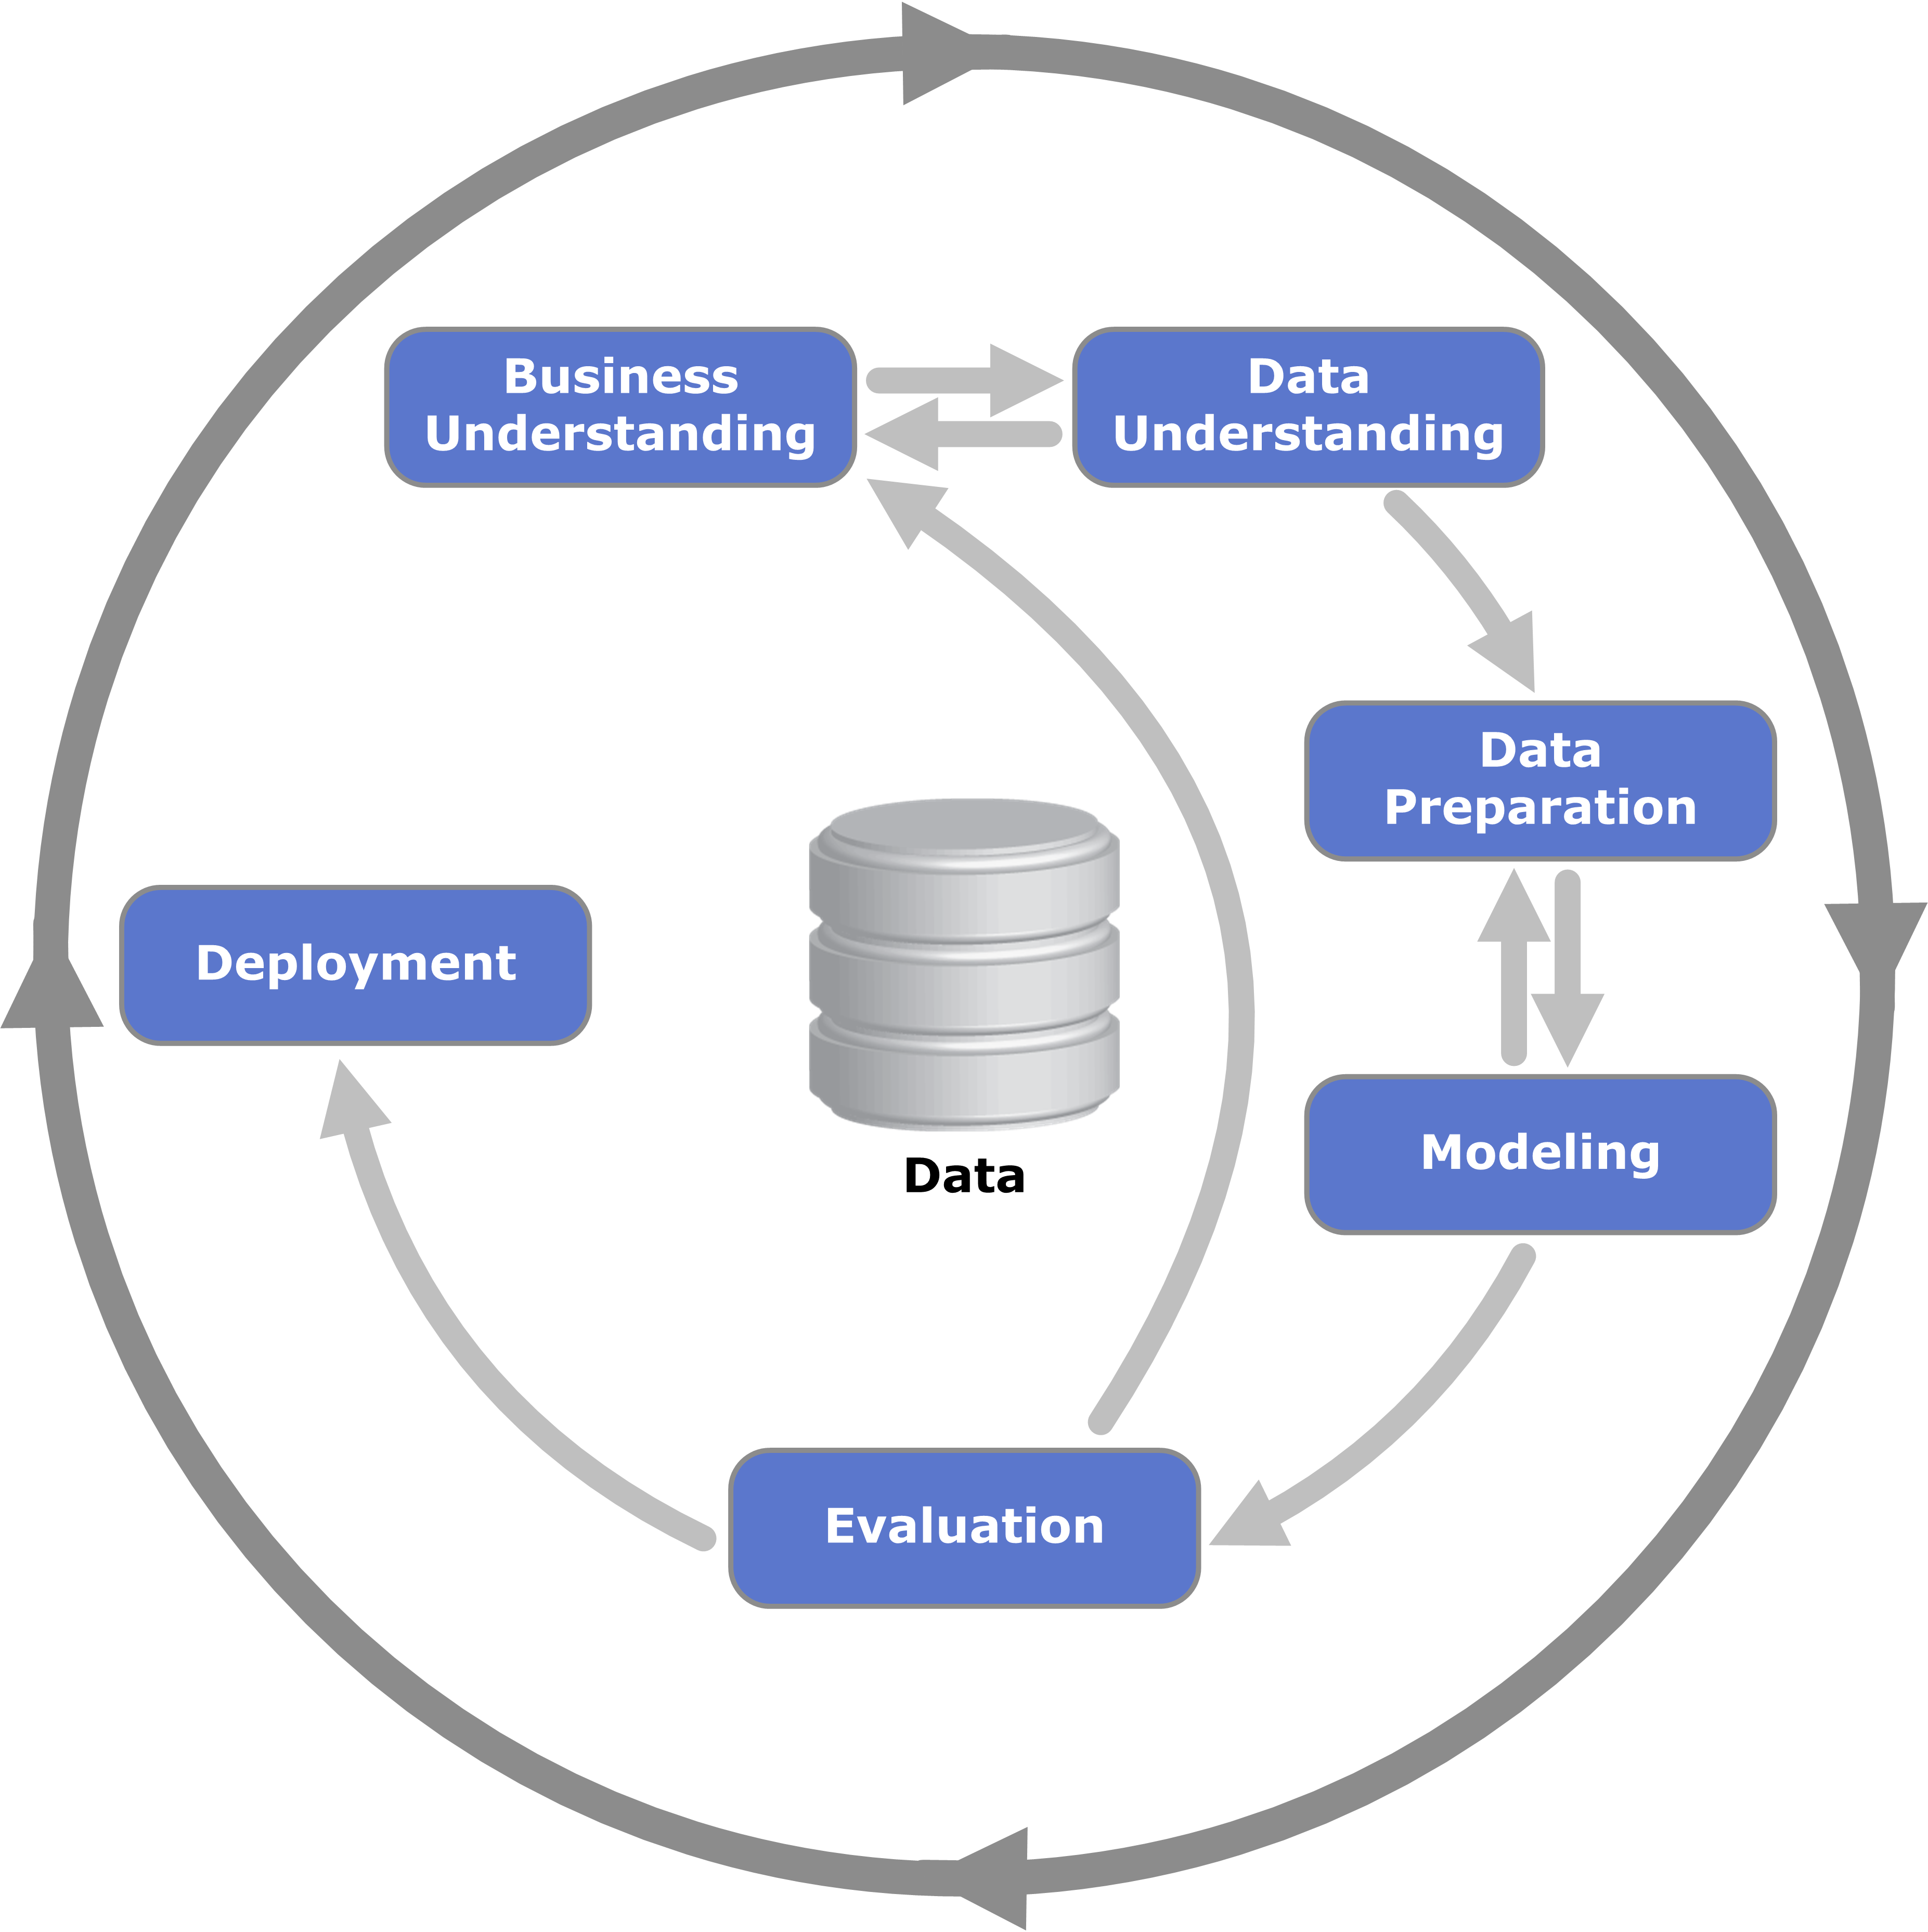
\includegraphics[width=0.65\textwidth]{diagrams/crisp_dm.png}
\caption{CRISP-DM lifecycle governing the project methodology and technical execution.}
\label{fig:methodology}
\end{figure}

As illustrated in Figure~\ref{fig:methodology}, the project methodology is governed by a circular CRISP-DM lifecycle that ensures rigorous technical execution across all steps. This framework specifically accommodates an iterative feedback loop between the evaluation and data preparation stages. Such a loop was essential for implementing Hard-Negative Mining in the Fire/Smoke dataset, allowing the system to continuously refine its understanding of challenging environmental artifacts and reduce false positive alerts.

For project tracking and collaboration, \textbf{GitHub} was used as the central platform, supporting version control and coordination of development activities.

\section{Chapter Summary}
This chapter presented the hosting organization (in2-Technologies) and the context of the EYE-D solution, then formalized the project overview, requirements, objectives, and the adopted project management approach. The next two chapters present the two implementation phases with their integrated state of the art studies, design diagrams, and implementation details under NPU deployment constraints. While general detection models provide a baseline, the specific safety requirements of industrial forklift tracking necessitate a transition toward real-time optimized architectures. Every algorithmic decision going forward is strictly evaluated against the limited SRAM and thermal thresholds of the target hardware. The following chapter details the selection and optimization of these models for NPU deployment.





